\chapter{Implementación}\label{cap:implementacion}
\Juanmi[]{Punto a revisar}

En este capítulo se describe la implementación del proyecto, así como detalles técnicos y decisiones tomadas durante el desarrollo. Se divide en varios sprints, cada uno con sus propias tareas y objetivos.

\section{Sprint 0}

En este sprint no se comienza el desarrollo del proyecto, sino que, como se menciona en la seccion \ref{cap:especificación} y \ref{cap:planificacion}, se realiza una investigación sobre las tecnologías a utilizar, y se detallan los requerimientos del sistema, y la arquitectura a implementar.
\newline\newline
Al usar Java (versión 21) como lenguaje de programación y Spring Boot (versión 3.4.4) como framework de desarrollo, se sigue un patrón similar para el desarrollo de los servicios, ya que todos comparten componentes y directorios similares.

\subsection{Estructura general de los servicios}

El código fuente de los servicios se organiza en paquetes, siguiendo una estructura común para todos los servicios. Esta estructura incluye:

\begin{itemize}
    \item \textbf{config}: Contiene la configuración del servicio, como la configuración de seguridad, bases de datos, etc.
    \item \textbf{controller}: Contiene los controladores REST que manejan las peticiones HTTP.
    \item \textbf{dto}: Contiene los objetos de transferencia de datos (DTO) utilizados para la comunicación entre el cliente y el servidor.
    \item \textbf{model}: Contiene las entidades del dominio del servicio.
    \item \textbf{repository}: Contiene las interfaces de repositorio que extienden de JPA para la persistencia de datos.
    \item \textbf{service}: Contiene la lógica de negocio del servicio.
    \item \textbf{mapper}: Contiene los mapeadores para convertir entre entidades y DTOs.
    \item \textbf{Application.java}: Clase principal que arranca el servicio.
\end{itemize}

De esta forma, se consigue una estructura clara y coherente para el desarrollo de los servicios, facilitando la comprensión y el mantenimiento del código.

Además para la configuración de estos, se utiliza un archivo de propiedades (application.properties) que permite definir las propiedades específicas del servicio, como la conexión a la base de datos, el puerto en el que se ejecuta el servicio, etc.

\section{Sprint 1}

Este primer sprint se comienza con cierta incertidumbre al no haber tenido todavía la reunión con Alberto Guillén Perales, el director del CEPRUD, por lo que no se sabe a qué información se va a tener acceso, y por tanto cómo se van a implementar ciertas funcionalidades.
\newline\newline
Sin embargo, ya que el proceso para poder hacer uso del sistema de autenticación de la UGR parece ser largo y requiere de una serie de permisos y pasos previos \cite{autenticacion_ugr}, se decide en este punto comenzar a implementar en el backend todas las funcionalidades relacionadas con la gestión de usuarios, y autenticación basadas en las credenciales de la UGR.
\newline\newline
Para conseguir esto se implementan los servicios ``User Service'', ``Auth Service'', ``Mail Service'' y el ``API Gateway''.

\subsection{User Service}

Este servicio se plantea como el encargado de gestionar los usuarios del sistema, permitiendo registrar, consultar, actualizar y eliminar usuarios. Además, se encarga de la gestión de roles y permisos, así como de la codificación de contraseñas.
\newline 
Las contraseñas se almacenan de forma segura mediante codificación (por ejemplo, \texttt{BCrypt}), y no en texto plano.
\newline\newline
Los usuarios pueden poseer los roles de \texttt{ROLE\_INACTIVE}, \texttt{ROLE\_STUDENT}, \texttt{ROLE\_TEACHER}, o \texttt{ROLE\_ADMIN}, y estos nos permiten controlar el acceso a diferentes funcionalidades del sistema.
\newline\newline
Aunque este servicio no es el encargado de la autenticación, srve de soporte para el servicio de autenticación, proporcionando la información de los usuarios y sus roles.

\subsubsection{Integración con otros microservicios}

\begin{itemize}
  \item Es consultado por otros servicios para validar identidad o permisos de los usuarios.
  \item Envía mensajes mediante RabbitMQ para notificar el registro de usuarios y/o cambios en sus credenciales.
\end{itemize}

\subsubsection{Diagrama de clases}
Este es el primer servicio implementado, y se sigue una estructura similar en los demás servicios para mantener la coherencia en el proyecto. La arquitectura de los servicios en la \textbf{Arquitectura limpia o hexagonal}, que se basa en la separación de responsabilidades y la independencia de las capas, se refleja en el diagrama de clases del servicio User Service, que se muestra en la figura \ref{fig:user-service-class-diagram}.
\begin{figure}[H]
    \centering
    \makebox[\textwidth][c]{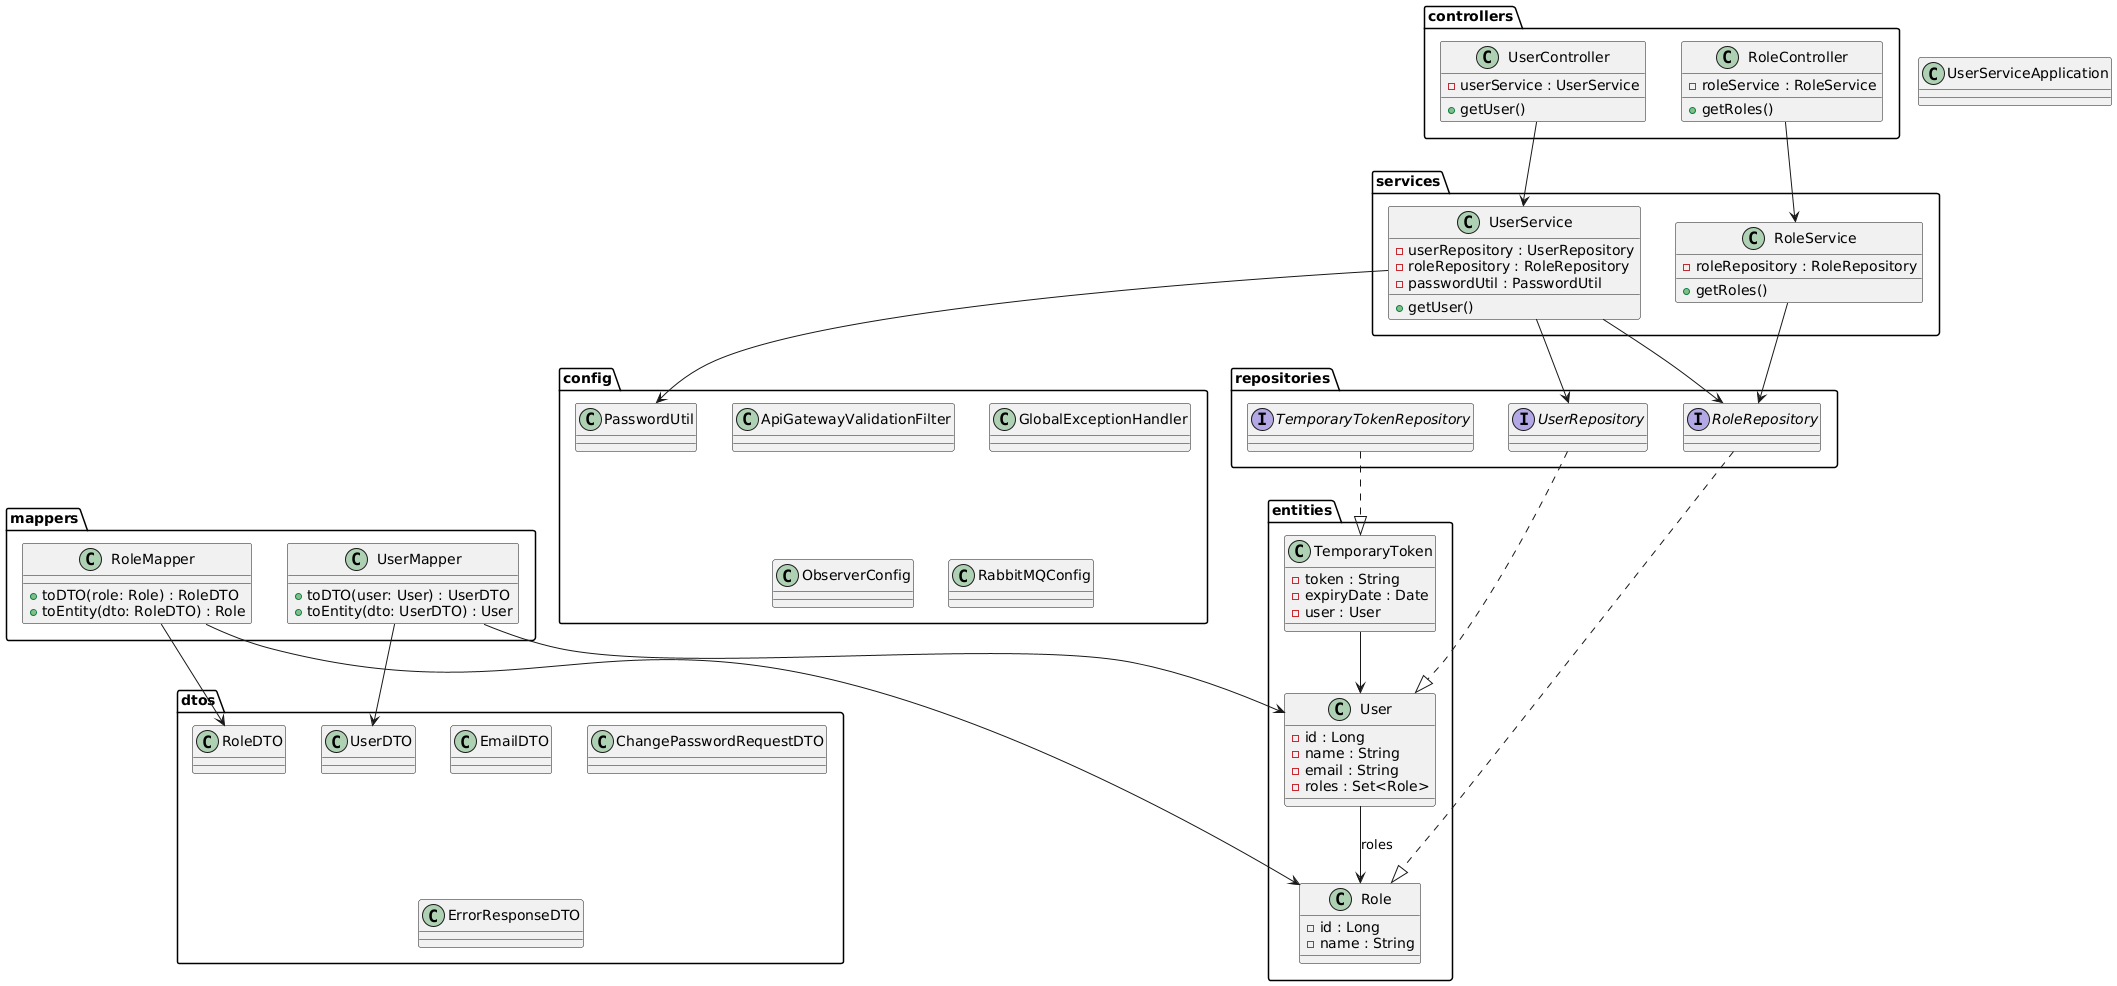
\includegraphics[width=1.2\textwidth]{figures/07_uml_user.png}}
    \caption{Diagrama de clases del servicio User Service realizado con PlantUML}
    \label{fig:user-service-class-diagram}
\end{figure}

Este diagrama representa las principales clases del servicio, incluyendo los controladores, servicios, repositorios y entidades. Cada clase tiene una responsabilidad clara y se comunica con otras clases a través de interfaces, lo que permite una fácil extensibilidad y mantenimiento del código.

\subsubsection{Interacción entre componentes}

\subsubsection*{1. Controladores (\texttt{controllers})}

\begin{itemize}
  \item \textbf{UserController} y \textbf{RoleController}: Son clases que exponen endpoints HTTP. Actúan como punto de entrada de las solicitudes del cliente.
  \item \textbf{Interacción}: Invocan métodos en los servicios correspondientes (\texttt{UserService}, \texttt{RoleService}) para obtener datos o ejecutar lógica de negocio.
\end{itemize}

\subsubsection*{2. Servicios (\texttt{services})}

\begin{itemize}
  \item \textbf{UserService}: Contiene la lógica de negocio relacionada con usuarios.
    \begin{itemize}
      \item Depende de \texttt{UserRepository} y \texttt{RoleRepository} para acceder a la base de datos.
      \item Usa \texttt{PasswordUtil} para tareas relacionadas con contraseñas (encriptación, validación, etc).
    \end{itemize}
  \item \textbf{RoleService}: Contiene lógica de negocio asociada a roles.
    \begin{itemize}
      \item Se comunica con \texttt{RoleRepository}.
    \end{itemize}
\end{itemize}

\subsubsection*{3. Repositorios (\texttt{repositories})}

\begin{itemize}
  \item \textbf{UserRepository}, \textbf{RoleRepository}, \textbf{TemporaryTokenRepository}: Son interfaces que definen operaciones CRUD (Create, Read, Update, Delete) sobre las entidades.
  \item \textbf{Interacción}: Son utilizados por los servicios para obtener o almacenar datos en la base de datos.
  Además toda la interacción con la base de datos se realiza a través de JPA, lo que permite una fácil integración y manejo de las entidades. JPA es un Objeto-Relational Mapping (ORM) que facilita la persistencia de datos en aplicaciones Java, permitiendo mapear clases Java a tablas de bases de datos relacionales.
\end{itemize}

\subsubsection*{4. Entidades (\texttt{entities})}

\begin{itemize}
  \item \textbf{User}: Representa un usuario del sistema. Tiene atributos como \texttt{id}, \texttt{name}, \texttt{email}, y una colección de \texttt{roles}.
  \item \textbf{Role}: Representa un rol o permiso dentro del sistema. Se relaciona con los usuarios.
  \item \textbf{TemporaryToken}: Usado para funcionalidades temporales como recuperación de contraseña. Contiene un \texttt{token}, una fecha de expiración y referencia al \texttt{User}.
  \item \textbf{Interacción}: Estas entidades son gestionadas por los repositorios y utilizadas en la lógica de negocio de los servicios.
\end{itemize}

\subsubsection*{5. Mapeadores (\texttt{mappers})}

\begin{itemize}
  \item \textbf{UserMapper} y \textbf{RoleMapper}: Se encargan de convertir entidades (\texttt{User}, \texttt{Role}) a sus correspondientes objetos de transferencia de datos (\texttt{UserDTO}, \texttt{RoleDTO}) y viceversa.
  \item \textbf{Interacción}: Usados por los servicios para traducir datos entre capas internas y externas.
\end{itemize}

\subsubsection*{6. DTOs (\texttt{dtos})}

\begin{itemize}
  \item \textbf{UserDTO}, \textbf{RoleDTO}, \textbf{EmailDTO}, \textbf{ChangePasswordRequestDTO}, \textbf{ErrorResponseDTO}: Representan estructuras de datos que se usan para enviar y recibir información a través de la API.
  \item \textbf{Interacción}: Son utilizados por los controladores y servicios para comunicar información de forma segura y controlada, evitando exponer entidades directamente.
\end{itemize}

\subsubsection*{7. Configuración (\texttt{config})}

\begin{itemize}
  \item \textbf{PasswordUtil}: Clase de utilidad para el manejo de contraseñas.
  \item \textbf{ApiGatewayValidationFilter}: Filtro que valida solicitudes entrantes desde el API Gateway.
  \item \textbf{GlobalExceptionHandler}: Captura y maneja excepciones globalmente.
  \item \textbf{RabbitMQConfig}, \textbf{ObserverConfig}: Configuración para mensajería y observadores (por ejemplo, eventos asincrónicos).
  \item \textbf{Interacción}: Algunas de estas clases son inyectadas en servicios (\texttt{PasswordUtil}), otras se ejecutan automáticamente (\texttt{GlobalExceptionHandler}).
\end{itemize}

\subsubsection*{8. Flujo de Interacción General}

\begin{enumerate}
  \item El cliente realiza una solicitud a través del \texttt{UserController} o \texttt{RoleController}.
  \item El controlador llama al servicio correspondiente (\texttt{UserService} o \texttt{RoleService}).
  \item El servicio accede a los repositorios para obtener datos desde las entidades.
  \item Se usan los mapeadores para convertir entidades en DTOs.
  \item El DTO es devuelto al cliente a través del controlador.
\end{enumerate}

Aunque en cada servicio se implementan diferentes funcionalidades, la estructura y la interacción entre los componentes siguen un patrón similar, lo que facilita la comprensión del código.
Para ilustrar de manera más simple lo detallado anteriormente, se muestra la figura \ref{fig:comm}, que representa la comunicación general entre los componentes del backend. 
\begin{figure}[H]
    \centering
    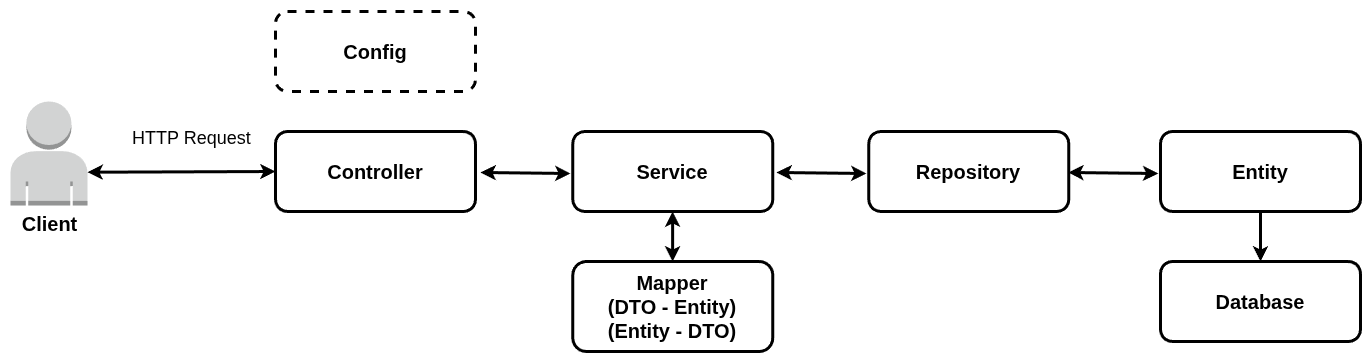
\includegraphics[width=0.95\textwidth]{figures/07_back.png}
    \caption{Comunicación general entre los componentes del backend}
    \label{fig:comm}
\end{figure}

\subsection{Mail Service}
El servicio de correo electrónico se encarga de enviar correos electrónicos a los usuarios del sistema. Este servicio es utilizado por otros servicios para enviar notificaciones, como la confirmación de registro, recuperación de contraseña, etc.

Su desarrollo combina tres tecnologías clave: \textbf{RabbitMQ}, \textbf{JavaMail} y \textbf{Thymeleaf}, permitiendo una integración fluida entre mensajería asíncrona y generación dinámica de contenido de correo.

El proceso comienza cuando otro componente del sistema necesita enviar un correo electrónico. En lugar de enviarlo directamente, publica un mensaje en una cola gestionada por \texttt{RabbitMQ}. Este servicio actúa como consumidor de esos mensajes mediante el uso de \texttt{listeners}, que reciben el contenido del mensaje en tiempo real. Esta estrategia permite desacoplar el proceso de envío de correo del resto de la lógica de negocio, mejorando la escalabilidad y la resiliencia del sistema ante posibles errores.

Una vez recibido el mensaje, el servicio extrae los datos necesarios, como la dirección de correo del destinatario, el asunto, y las variables que se inyectarán en el contenido. Para la composición del cuerpo del correo, se utiliza \texttt{Thymeleaf}, un motor de plantillas que permite construir correos HTML personalizados. Gracias a Thymeleaf, se pueden generar correos enriquecidos visualmente, dinámicos y adaptados al contexto de cada notificación, manteniendo una presentación clara y profesional.

Después de generar el contenido del correo, se utiliza la biblioteca \texttt{JavaMail} para su envío. JavaMail proporciona una API robusta y configurable que permite construir mensajes MIME, manejar los encabezados, adjuntos y establecer la conexión con el servidor SMTP. En este caso, se ha configurado el servicio para utilizar \textbf{Gmail como proveedor de correo electrónico}, lo cual requiere definir parámetros como el host SMTP de Gmail (\texttt{smtp.gmail.com}), el puerto correspondiente, y habilitar la autenticación y conexión segura mediante TLS. Esta configuración se especifica en los archivos de propiedades del servicio, lo que facilita su adaptación a distintos entornos de despliegue.

En conjunto, este microservicio representa una solución elegante y modular para el envío de correos~\ref{fig:mail-service-class-diagram} en arquitecturas basadas en microservicios. Aprovecha la comunicación asincrónica de RabbitMQ, la potencia expresiva de las plantillas Thymeleaf, y la fiabilidad de JavaMail para lograr un sistema de notificaciones por correo eficaz, personalizable y mantenible.

\begin{figure}[H]
    \centering
    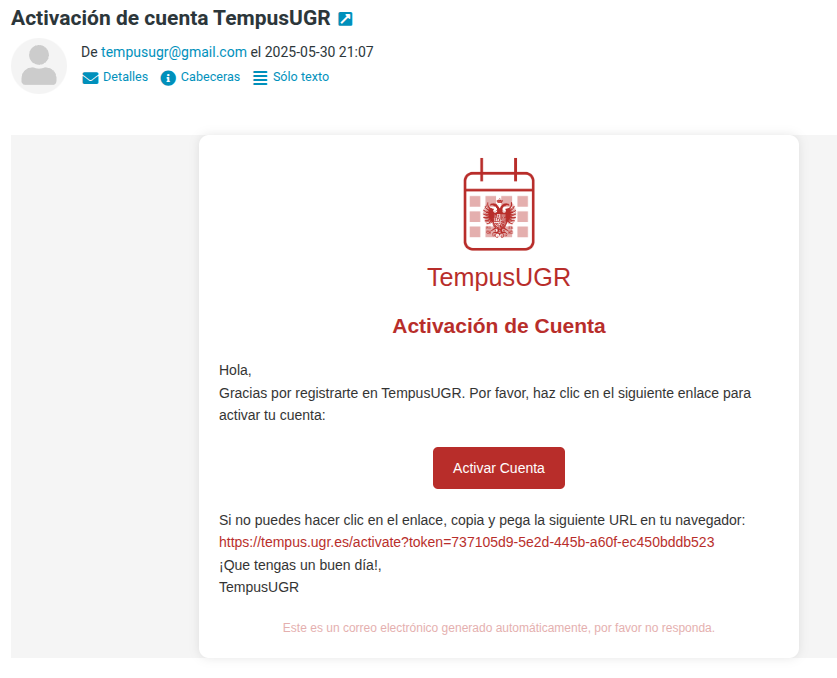
\includegraphics[width=0.8\textwidth]{figures/07_email.png}
    \caption{Correo de activación de cuenta}
    \label{fig:mail-service-class-diagram}
\end{figure}

\subsection{Auth Service}
El servicio de autenticación es el encargado de gestionar la autenticación de los usuarios del sistema. Este servicio se encarga de validar las credenciales de los usuarios y generar tokens JWT (JSON Web Tokens) para autenticar las solicitudes a otros servicios.
\newline\newline
Su lógica reside en la clase \texttt{AuthService}. 
La operación principal, \texttt{authenticate}, recibe las credenciales enviadas por el cliente y devuelve un par de tokens
\emph{JSON Web Token} (JWT): un \emph{access token} de corta duración y un \emph{refresh token} de duración más amplia. 

El proceso comienza verificando que la dirección de correo pertenezca a la Universidad de Granada; 
de lo contrario, se aborta la autenticación.  
Después, mediante un \texttt{WebClient} reactivo, el servicio consulta al microservicio de usuarios 
(\texttt{user-service}) para recuperar el \texttt{UserDTO} correspondiente.  
Si el usuario existe, está activo y la contraseña coincide con el \emph{hash} almacenado (comprobación
delegada a \texttt{PasswordUtil}), se generan ambos tokens.

\subsubsection*{Estructura del JWT}

Un JWT es una cadena en tres partes \emph{``header.payload.signature''}, codificadas en \texttt{Base64Url}.  
En este servicio se firma con el algoritmo simétrico \texttt{HS256}, usando la clave secreta
\lstinline|JWT_SECRET|:

\begin{verbatim}
Key key = Keys.hmacShaKeyFor(SECRET_KEY.getBytes(StandardCharsets.UTF_8));
String jwt = Jwts.builder()
        .setHeaderParam("typ", "JWT")
        .setSubject(id)              // Identificador del usuario
        .claim("role", role)         // Rol de la aplicación
        .setIssuedAt(new Date(now))
        .setExpiration(new Date(now + ttl))
        .signWith(key, SignatureAlgorithm.HS256)
        .compact();
\end{verbatim}

La cabecera (\texttt{header}) indica el tipo de token y el algoritmo de firma.  
El cuerpo (\texttt{payload}) almacena el identificador del usuario (\texttt{sub}), su rol y las marcas
temporal de emisión y caducidad (\texttt{iat}, \texttt{exp}).  
La firma garantiza la integridad: si cualquier byte del token cambia, la verificación falla.

\subsubsection*{Duración y refresco}

El \emph{access token} caduca en 24~horas (86,400,000~ms), su vida corta limita el riesgo ante robo.  
El \emph{refresh token} dura una semana y sólo sirve para
obtener nuevos \emph{access tokens}.  
La operación \texttt{refresh} valida la firma y la vigencia del \emph{refresh token};  
si supera la comprobación, crea un nuevo \emph{access token} manteniendo el \emph{refresh token} 
original mientras no haya expirado.  
El servidor no almacena sesiones, por lo que el mecanismo es \emph{stateless} y escalable: basta con
compartir la misma \lstinline|JWT_SECRET| entre las instancias.

\subsubsection*{Flujo de autenticación}

El diseño evita guardar estado en la base de datos y permite balancear las peticiones entre múltiples
réplicas sin afinidad de sesión.  

El flujo de autenticación y generación de tokens JWT se ilustra en la figura \ref{fig:auth-service-class-diagram}, donde se muestra cómo el servicio interactúa con el \texttt{user-service} para validar las credenciales y generar los tokens necesarios.

\begin{figure}[H]
    \centering
    \makebox[\textwidth][c]{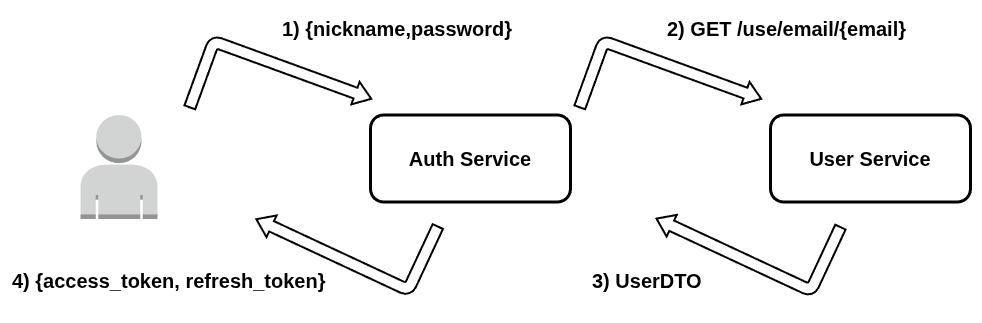
\includegraphics[width=1.1\textwidth]{figures/07_auth.png}}
    \caption{Flujo de autenticación y generación de tokens JWT}
    \label{fig:auth-service-class-diagram}
\end{figure}

\subsection{API Gateway}
El \texttt{api-gateway} actúa como el punto de entrada centralizado para todas las peticiones del sistema basado en microservicios. Está construido utilizando \textbf{Spring Cloud Gateway}, una solución reactiva que permite enrutar solicitudes a los distintos servicios internos, como \texttt{user-service} o \texttt{auth-service}. Su función no se limita al enrutamiento, sino que también gestiona aspectos transversales como la seguridad, la autenticación mediante JWT, y la validación de rutas públicas y protegidas.

\subsubsection{Spring Security en el Gateway}

\textbf{Spring Security} es un framework de seguridad potente y altamente configurable, que se utiliza para proteger tanto aplicaciones monolíticas como distribuidas. En el contexto del \texttt{api-gateway}, se emplea para interceptar las peticiones entrantes y aplicar mecanismos de autenticación antes de permitir el acceso a los servicios internos. Aquí no se gestionan sesiones, sino que se trabaja con tokens JWT (JSON Web Tokens), que son validados en cada petición.

El archivo \texttt{SecurityConfig} define la configuración de seguridad. En este componente se especifican:
\begin{itemize}
  \item Los filtros personalizados que deben ejecutarse antes del procesamiento de cada solicitud.
  \item Las rutas que deben ser públicas (por ejemplo, el login o el registro).
  \item Que el sistema funciona sin sesiones, usando una política \texttt{stateless}.
\end{itemize}

\subsubsection{Filtros personalizados}

Spring Security permite encadenar filtros que procesan las solicitudes antes de llegar a los controladores. En el gateway, se implementan dos filtros principales:

\paragraph{JwtAuthenticationFilter} Este filtro se encarga de interceptar todas las solicitudes entrantes y validar que el JWT (token de acceso) esté presente y sea válido. Para ello, extrae el token del encabezado \texttt{Authorization} y realiza una verificación utilizando una clave secreta compartida. En caso de éxito, el filtro añade los atributos del usuario autenticado al encabezado de la petición, de modo que los servicios internos puedan conocer la identidad y rol del usuario. Si el token no es válido o está ausente, la solicitud se rechaza con un error HTTP \texttt{401 Unauthorized}.

\paragraph{PathPrefixFilter} Elimina el prefijo /calendarugr/v1 de la ruta de cada petición entrante en el API Gateway. Si la URL comienza con ese prefijo, lo elimina y reescribe la ruta antes de pasar la petición al siguiente filtro o servicio interno. Así, los microservicios reciben rutas limpias y sin el prefijo de versión, facilitando el enrutamiento interno. Además, el filtro tiene la máxima prioridad para ejecutarse antes que otros filtros de seguridad.

\subsubsection{Configuración de rutas seguras}

En el archivo de configuración \texttt{SecurityConfig}, se define explícitamente qué rutas deben estar protegidas. Por ejemplo, aquellas que comienzan con \texttt{/user} pueden requerir un token JWT válido, mientras que rutas como \texttt{/auth/login} son públicas. Esta distinción permite implementar un control de acceso granular a través del propio gateway, centralizando así la lógica de seguridad.

Además, se utiliza una política de seguridad sin estado (\texttt{SecurityContextHolder.MODE\_INHERITABLETHREADLOCAL}) y se desactivan los mecanismos tradicionales como CSRF y sesiones HTTP, ya que todo el control de identidad se realiza mediante tokens.

En resumen, el \texttt{api-gateway} cumple un rol esencial en la arquitectura del sistema, actuando no solo como un proxy inverso, sino también como un punto de control de acceso. Gracias a Spring Security y a los filtros como \texttt{JwtAuthenticationFilter}, se logra una protección robusta y centralizada, adecuada para entornos distribuidos donde cada microservicio es independiente pero requiere información sobre la identidad del usuario que realiza la petición.

\subsection{RabbitMQ}
El servicio de mensajería RabbitMQ se integra en el sistema para facilitar la comunicación asíncrona entre los diferentes microservicios. Este enfoque permite desacoplar los servicios, mejorar la escalabilidad y manejar picos de carga sin afectar la disponibilidad del sistema.
\subsubsection{Configuración de RabbitMQ}
RabbitMQ se configura en el archivo \texttt{application.properties} de cada servicio que lo utiliza. Se especifican parámetros como el host del servidor RabbitMQ, el puerto, el nombre de usuario y la contraseña.
\subsubsection{Funcionamiento de RabbitMQ}

RabbitMQ es un sistema de mensajería basado en el modelo \textit{message broker}, que permite la comunicación asíncrona entre distintos servicios. Se apoya en el protocolo AMQP (\textit{Advanced Message Queuing Protocol}), un protocolo binario de capa de aplicación diseñado para asegurar la interoperabilidad entre sistemas, fiabilidad en la entrega de mensajes y soporte para confirmaciones, encolado y reintentos.

En una arquitectura de microservicios, RabbitMQ permite desacoplar componentes mediante el intercambio de mensajes a través de colas. Un servicio puede publicar un mensaje sin necesidad de que el receptor esté disponible en ese momento. Esta estrategia mejora la tolerancia a fallos y la escalabilidad del sistema.

\subsubsection{Componentes principales}

RabbitMQ se basa en cuatro componentes clave:

\begin{itemize}
  \item \textbf{Productores (Producers)}: servicios que envían mensajes. En este caso, el \texttt{user-service} actúa como productor.
  \item \textbf{Intercambios (Exchanges)}: puntos intermedios que reciben mensajes y los redirigen a una o más colas basándose en reglas de enrutamiento. Existen varios tipos, como \texttt{direct}, \texttt{fanout}, \texttt{topic} y \texttt{headers}.
  \item \textbf{Colas (Queues)}: estructuras donde los mensajes son almacenados hasta que un consumidor los procesa.
  \item \textbf{Consumidores (Consumers)}: servicios que reciben y procesan los mensajes. En este caso, el \texttt{mail-service} es el consumidor.
\end{itemize}

\subsubsection{Configuración en \texttt{user-service}}

El servicio \texttt{user-service} actúa únicamente como productor. Su configuración en \texttt{RabbitMQConfig} define un \texttt{DirectExchange} llamado \texttt{mail\_exchange}, y una clave de enrutamiento \texttt{registering\_routing\_key}. Esto implica que todos los mensajes enviados desde este servicio se publican a dicho \texttt{exchange} con esa clave.

\begin{verbatim}
DirectExchange exchange() {
    return new DirectExchange("mail_exchange");
}
\end{verbatim}

Este fragmento configura el punto de entrada de los mensajes que serán enviados al sistema de mensajería.

\subsubsection{Configuración en \texttt{mail-service}}

El servicio \texttt{mail-service} funciona exclusivamente como consumidor de mensajes~\ref{fig:rabbitmq-config}. Su configuración es más extensa, ya que debe definir tanto las colas como las asociaciones con el intercambio, además de políticas de reintento y manejo de errores.

Se definen dos colas principales:
\begin{itemize}
  \item \texttt{registering\_queue}, para correos de confirmación de registro.
  \item \texttt{notification\_queue}, para notificaciones genéricas.
\end{itemize}

Ambas están enlazadas al \texttt{mail\_exchange} mediante sus respectivas claves de enrutamiento. Esta asociación se realiza mediante \texttt{Binding}.

También se especifica un convertidor de mensajes para que RabbitMQ utilice JSON como formato de serialización, mediante \texttt{Jackson2JsonMessageConverter}, permitiendo la compatibilidad con objetos Java.

\begin{figure}[H]
    \centering
    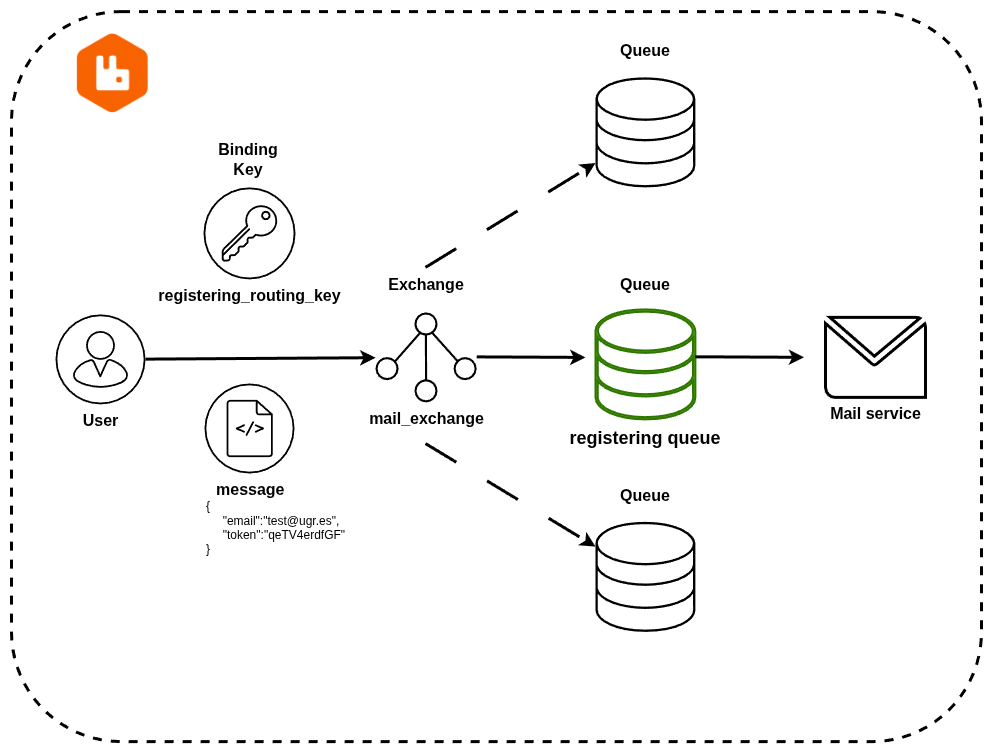
\includegraphics[width=0.8\textwidth]{figures/07_rabbit.png}
    \caption{Configuración de RabbitMQ en el servicio mail-service}
    \label{fig:rabbitmq-config}
\end{figure}

\subsubsection{Reintentos automáticos y Dead Letter Queues}

Una característica importante de la configuración es la gestión de reintentos automáticos y colas de mensajes muertos (DLQ).

Los reintentos se configuran a través de un \texttt{RetryInterceptor}:
\begin{verbatim}
.maxAttempts(3)
.backOffOptions(1000, 2.0, 50000)
\end{verbatim}
Esto indica que, si el procesamiento de un mensaje falla, se reintentará hasta tres veces, con un intervalo inicial de 1 segundo y un multiplicador exponencial. Si después de los reintentos no se logra procesar el mensaje, este se considera fallido.

En lugar de eliminar estos mensajes fallidos, se redirigen a una \textbf{Dead Letter Queue}, en este caso \texttt{mail\_dead\_letter\_queue}, asociada a su propio \texttt{Dead Letter Exchange} (\texttt{mail\_dead\_letter\_exchange}). Esto permite su análisis posterior, ya sea manual o mediante herramientas automáticas.

\subsubsection{Resumen funcional}

En este sistema, el \texttt{user-service} publica eventos de registro de usuarios a RabbitMQ. El \texttt{mail-service} escucha la cola correspondiente y envía los correos pertinentes. En caso de fallos temporales, se aplican políticas de reintento. Si el fallo persiste, el mensaje es redirigido a una DLQ, asegurando que ningún mensaje se pierde sin ser registrado.

Esta estrategia desacopla los servicios, mejora la resiliencia del sistema, y permite manejar errores de forma controlada sin interrumpir el flujo principal de la aplicación.

\subsection{Primer hito del backend}
El primer hito del backend se alcanza con la implementación de los servicios de autenticación y gestión de usuarios, junto con el servicio de correo electrónico. Estos servicios permiten registrar usuarios, autenticar sus credenciales y enviar correos electrónicos de confirmación. Además, se ha implementado el API Gateway para centralizar las peticiones y gestionar la seguridad mediante JWT.
\newline\newline
El siguiente paso antes de comenzar el siguiente sprint, y tras la reunión con Alberto Guillén Perales, es investigar cómo se pueden obtener los horarios de las asignaturas de la UGR.
\newline\newline
Para ello se investiga el sistema de scrapping, y se implementa un primer prototipo que permite obtener los horarios de las asignaturas de la UGR. Este prototipo se implementa en una primera aproximación del servicio \texttt{schedule-consumer-service}, que se encargará de consumir los horarios de las asignaturas y generar eventos a partir de ellos.
\newline
La tecnología seleccionada para realizar la tarea de scrapping es \textbf{Jsoup}, una biblioteca de Java que permite extraer y manipular datos de documentos HTML. Jsoup proporciona una API sencilla para navegar por el DOM, seleccionar elementos y extraer información, lo que facilita la tarea de scrapping.

\subsubsection{Scrapping con Jsoup}

El sistema realiza un proceso de extracción automatizado desde un portal académico para recopilar información sobre titulaciones, asignaturas, profesorado, grupos y horarios, utilizando técnicas de \textit{web scraping} con la biblioteca \texttt{Jsoup} y almacenamiento en base de datos mediante repositorios JPA.

La primera fase del proceso consiste en acceder al portal principal de ramas de conocimiento, desde donde se extraen los enlaces hacia las distintas titulaciones. A partir de cada enlace, se accede a la página específica de la titulación y se recogen sus datos básicos. Si la titulación no está ya registrada en la base de datos, se crea una nueva entrada con su nombre, URL y rama correspondiente.

Posteriormente, se recorre cada titulación almacenada y se accede a su página detallada para obtener dos tipos de información. Por un lado, si no se ha registrado la facultad correspondiente, se extrae de una tabla presente en el sitio web. Por otro lado, se recopilan los enlaces de todas las asignaturas que pertenecen a dicha titulación. Estas asignaturas se crean en la base de datos sólo si no existen previamente, y se asocian con la titulación correspondiente.

La última fase del proceso accede a cada una de las asignaturas almacenadas para extraer información detallada. En primer lugar, se recoge la información general de la asignatura como el curso académico, el año, el semestre, el tipo y el departamento responsable. Se aplican medidas de control como el recorte del texto del departamento si excede una longitud determinada.

Después, se identifica al profesorado vinculado a la asignatura y a sus respectivos grupos. Si el grupo ya existe, se actualiza su lista de profesores. Si no existe, se crea y se almacena junto con el nombre del profesor. Se contempla la posibilidad de que algunos grupos no aparezcan explícitamente en la web, en cuyo caso se generan automáticamente.

Finalmente, se extrae el horario de clases para cada grupo, identificando el día de la semana, aula, fechas de inicio y fin, y horas de inicio y fin. Esta información se transforma en objetos de clase que se asocian con el grupo correspondiente. Si no se detecta una clase idéntica en la base de datos, se crea una nueva entrada para ella.

Este enfoque~\ref{fig:scrapping-process} permite consolidar una base de datos académica completa, dinámica y precisa, ideal para ser explotada por nuestro sistema.

%figura de scrapping, recortar un poco por arriba
\begin{figure}[H]
    \centering
    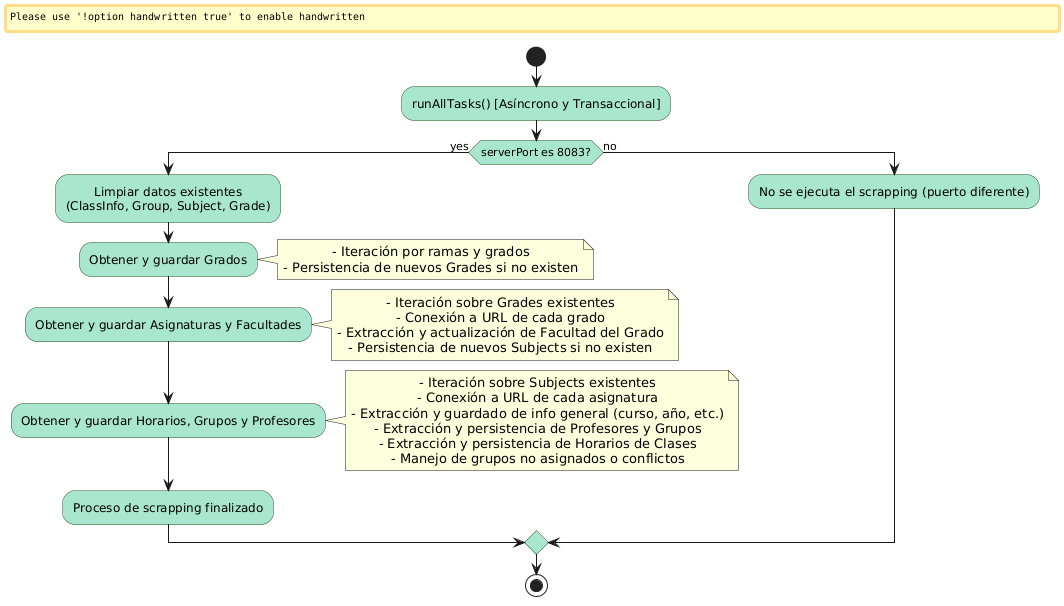
\includegraphics[width=1\textwidth, trim=0 0 0 45, clip]{figures/07_scrapping.png}
    \caption{Proceso de scrapping de asignaturas y horarios}
    \label{fig:scrapping-process}
\end{figure}

\section{Sprint 2}

En el comienzo de este sprint se continúa afinando y completando el script de scrapping, y revisando que se recoja información de todos los grados y asignaturas de la UGR. Esto se consigue realizando una labor de análisis exhaustivo de las diferenmtes páginas y secciones que conforman el portal de ``grados UGR'' mencionado con anterioridad.
\subsubsection{Schedule Consumer Service}
Paralelo a este desarrollo, se comienza el desarrolo del servicio \texttt{schedule-consumer-service}. Este es el encargado de, en primer lugar, hacer uso del scrapping para obtener los horarios de las asignaturas y almacenar la información en la base de datos, y en segundo lugar, de exponer endpoints relacionados con la consulta de estos datos. Uno de los objetivos de la realización se este servicio es poseer endpoints públicos para poder ser consumidos desde otros sistemas externos a nuestro frontend ``TempusUGR''.
\newline\newline
Una vez hecho el scrapping, y la información en base de datos (integrando el script de scrapping con el resto de componentes de Spring como lo son ``Repositories'',''Controllers'', etc), se necesita una manera de actualización de la información, puesto que es una de las premisas del sistema, mantener un acceso personalizado y actualizado del calendario académico.\newline
Para conseguir esto, y puesto que iterar y comprobar cambios sobre las más de 50.000 clases distintas impartidas en grupos de asignatura de la UGR es una tarea costosa y compleja, se decide implementar un ``\hypertarget{cronjob}{Cron job}'' que se encargue de realizar el scrapping de forma periódica, y así mantener la información actualizada. Este cron job se implementa en el servicio \texttt{schedule-consumer-service} y se ejecuta todos los días a las 00:00 horas, de forma que se actualizan los horarios de las asignaturas y se eliminan aquellos que ya no existen.
\newline\newline
Spring Boot proporciona una forma sencilla de implementar cron jobs mediante la anotación \texttt{@Scheduled}. Esta anotación permite definir un método que se ejecutará periódicamente según una expresión cron. En este caso, se ha configurado para que el método de actualización de horarios se ejecute diariamente a medianoche. Además de la anotación \texttt{@Scheduled}, se utiliza la anotación \texttt{@EnableScheduling} en la clase de configuración principal del servicio para habilitar el soporte de programación de tareas, y la anotación \texttt{@Async} para permitir la ejecución asíncrona de los métodos, lo que mejora la eficiencia y la capacidad de respuesta del servicio.
\newline
Para evitar un fallo del funcionamiento del servicio mientras se realiza una sustitución de los datos (Primero se borran los horarios antiguos, y luego se añaden los nuevos), se hace uso también de la anotación \texttt{@Transactional}, proveniente de ``Spring Transaction'', en el método que realiza la actualización de horarios. Esto asegura que todas las operaciones de base de datos se realicen dentro de una transacción, lo que garantiza la consistencia de los datos y evita problemas de concurrencia. Así los usuarios pueden seguir consultando la información de horarios sin  interrupciones, incluso durante el proceso de actualización.
\newline\newline
Una vez implementado el servicio se consigue el servicio troncal del backend, que permite obtener los horarios de las asignaturas de la UGR, y exponerlos a través de una API REST. Este servicio se convierte en el núcleo del sistema, ya que proporciona la información necesaria para el objetivo principal del proyecto: ofrecer un calendario académico personalizado y actualizado para los estudiantes de la UGR.

\subsubsection{Academic Subscription Service}
Así se comienza con el desarrollo del servicio \texttt{academic-subscription-service}, que se encargará de gestionar las suscripciones a los grupos de asignaturas de cualquier grado de la UGR.\newline
Las suscripciones se componen del identificador del usuario, la facultad, el grado, la asignatura y su grupo, puesto que de otra manera no se podría identificar de forma única un grupo de asignatura, ya que puede haber grupos con el mismo nombre en diferentes grados o facultades. Con esta información se hacen peticiones al servicio \texttt{schedule-consumer-service} para obtener los horarios de las asignaturas~\ref{classes} y generar un calendario personalizado para el usuario con sus clases oficiales.\newline

\begin{figure}[H]
    \centering
    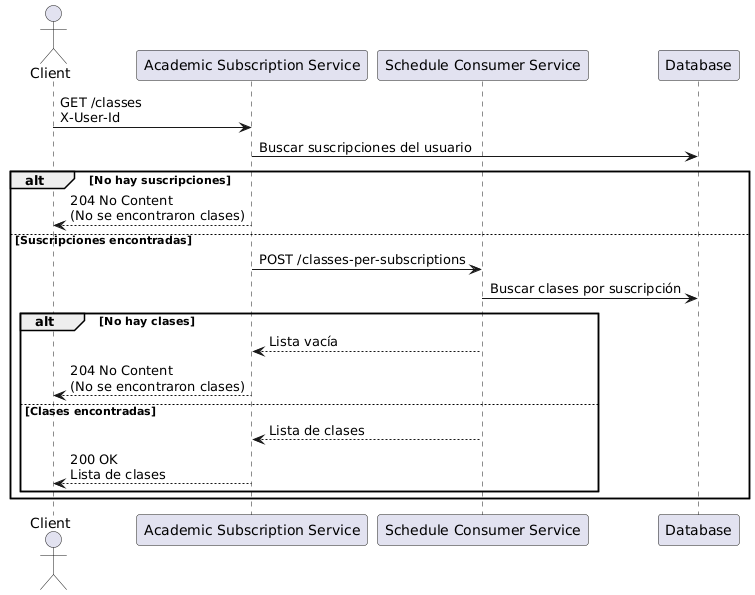
\includegraphics[width=0.95\textwidth]{figures/07_classes.png}
    \caption{Servicio de suscripciones académicas}
    \label{classes}
\end{figure}

Una vez se consigue esta información en formato ``JSON'', se implementa la lógica para generar un archivo \texttt{.ics}\cite{icalendar} que pueda ser importado en aplicaciones de calendario como Google Calendar, Outlook, etc. Para ello se utiliza la biblioteca \texttt{ical4j}, que permite crear y manipular archivos de calendario en formato iCalendar (\texttt{.ics}).\newline
\newline
Para crear esta primera versión de ``.ics'' se hace uso de los eventos recurrentes ( \texttt{RRULE}) de iCalendar, que permiten definir patrones de repetición para eventos. Esto es especialmente útil para las clases que se repiten semanalmente, ya que permite definir una sola entrada en el calendario que se repetirá automáticamente en las fechas correspondientes.\newline
\newline
Toda la información en este servicio se almacena en una base de datos no relacional, en este caso \texttt{MongoDB}, que permite una mayor flexibilidad y escalabilidad para almacenar los datos de las suscripciones y los horarios de las asignaturas. 

\subsubsection{Eureka Discovery Server}
A esta altura del proyecto en la que ya se tienen desarrollados varios servicios, se decide implementar un servidor de descubrimiento de servicios utilizando \textbf{Eureka}, que es parte del ecosistema de Spring Cloud. Eureka permite a los servicios registrarse y descubrir otros servicios en el sistema, facilitando la comunicación entre ellos sin necesidad de conocer sus direcciones IP o puertos específicos.
\newline 
Para conseguir esto se crea un nuevo proyecto de Spring Boot que actúa como el servidor Eureka. Este servidor se configura para permitir que otros servicios se registren y descubran entre sí. Cada servicio que se desea registrar en Eureka debe incluir la dependencia de \texttt{spring-cloud-starter-netflix-eureka-client} y configurarse adecuadamente en su archivo \texttt{application.properties}.
\newline
Esto nos permite los siguientes avances:
\begin{itemize}
  \item \textbf{Balanceo de carga}: Al registrar los servicios en Eureka, se pueden utilizar balanceadores de carga de manera dinámica, sin necesidad de configurar manualmente las direcciones IP y puertos de cada servicio. Eureka proporciona una lista de instancias disponibles, lo que permite al cliente elegir una instancia para enviar la solicitud.
  \item \textbf{Alta disponibilidad}: Si un servicio falla, Eureka permite que otros servicios sigan funcionando sin interrupciones, ya que pueden redirigir las peticiones a otras instancias disponibles.
  \item \textbf{Configuración centralizada}: Permite gestionar la configuración de los servicios desde un único punto, facilitando el mantenimiento y la actualización del sistema.
  \item \textbf{Facilidad de desarrollo}: Al utilizar Eureka, los desarrolladores pueden centrarse en la lógica de negocio de sus servicios sin preocuparse por la gestión de direcciones IP y puertos, ya que Eureka se encarga de ello. Es decir, las llamadas HTTP pasan de tener un formato similar a este \texttt{http://localhost:8081/calendarugr/v1/user-service/users} a \texttt{http://user-service/users}, donde \texttt{user-service} es el nombre del servicio registrado en Eureka.
\end{itemize}

De esta manera podemos tener un control de los servicios que se están ejecutando en el sistema~\ref{eureka}, y facilitar la comunicación entre ellos. Además, se puede escalar horizontalmente los servicios, añadiendo más instancias de un mismo servicio sin necesidad de modificar el código del cliente.

\begin{figure}[H]
    \centering
    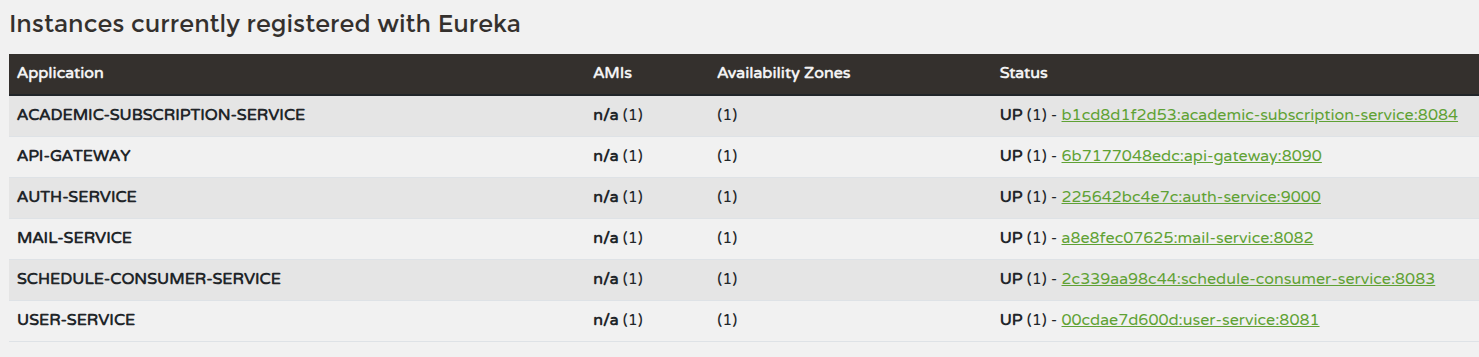
\includegraphics[width=1\textwidth]{figures/07_eureka.png}
    \caption{Servidor de descubrimiento de servicios con Eureka}
    \label{eureka}
\end{figure}

\section{Sprint 3}

El comienzo de estas tres semanas estuvo centrado en la finalización del servicio \texttt{academic-subscription-service}, que se encarga de gestionar las suscripciones a los grupos de asignaturas de cualquier grado de la UGR.\newline
Para conseguir esto, se implementa la gestión de eventos a nivel de grupo (eventos que son relevantes para aquellas personas suscritas a ese grupo de asignatura), y eventos a nivel de facultad (eventos que son relevantes para todas las personas suscritas a cualquier grupo de asignatura de esa facultad). Estos eventos se almacenan en la base de datos del servicio \texttt{academic-subscription-service}, en una tabla diferente a las suscripciones.\newline
Para poder crear estos eventos, el usuario debe ser tanto profesor como administrador, y para poder crear eventos a nivel de facultad, el usuario debe ser administrador. Estos eventos se crean a través de endpoints del servicio \texttt{academic-subscription-service}. 
\newline\newline
Una vez se crean los eventos, estos serán visibles para todos los usuarios suscritos a ese grupo de asignatura o facultad, y se enviarán notificaciones a través del servicio de correo electrónico (\texttt{mail-service}) a todos los usuarios suscritos con notificaciones activadas. Estas notificaciones se envían mediante RabbitMQ, como se ha explicado anteriormente, y se generan correos electrónicos personalizados utilizando plantillas Thymeleaf en el servicio de mail.
\newline\newline
Una vez creados los eventos, e implementada la posibilidad de poder obtener la información de estos y clases oficiales, se adaptó la creación de los archivos \texttt{.ics} para incluir tanto las clases oficiales como los eventos de grupo y facultad. Estos al contrario que las clases oficiales, no son recurrentes, por lo que se crean como eventos únicos en el calendario. De esta manera, el usuario puede importar un archivo \texttt{.ics} que contenga tanto sus clases oficiales como los eventos de grupo y facultad a su calendario personal, ya sea Google Calendar, Outlook, etc.\newline
\newline\newline
Además de esto se implementa la sincronización con Google Calendar. Para conseguir esto se pueden seguir diferentes estrategias:
\begin{itemize}
  \item \textbf{Google Calendar API}: Utilizar la API de Google Calendar para crear eventos directamente en el calendario del usuario. Esto requiere que el usuario autorice la aplicación a acceder a su calendario.
  \item \textbf{Exportación de archivos ICS}: Generar un archivo \texttt{.ics} que el usuario pueda descargar e importar manualmente en su Google Calendar.
  \item \textbf{Url de sincronización}: Proporcionar una URL de suscripción a un calendario que Google Calendar pueda utilizar para sincronizar automáticamente los eventos y clases oficiales.
\end{itemize}

En este caso, y como el sistema ya requiere el correo institucional al usuario (con el de google no podemos descifrar si es estudiante o docente), se opta por la tercera opción, que es la más sencilla y permite al usuario sincronizar su calendario de forma automática. Para ello se genera una URL que el usuario puede añadir a su Google Calendar, y que se actualizará automáticamente con los eventos y clases oficiales del usuario.
El acceso a esta URL es público, por lo que cualquier persona que tenga el enlace podrá acceder a los eventos y clases oficiales del usuario. Esto se decide hacer de esta manera para que Google Calendar pueda acceder a la información sin necesidad de autenticación, ya que el usuario ya ha autorizado la aplicación a acceder a su calendario al momento de crear la suscripción.
\newline
La fabricación de esta URL requiere la creación de un hash único para cada usuario que además sea ``reversible'' para identificar la pertenencia del mismo. Para conseguir esto se hizo uso de ``AES'', un algoritmo de cifrado simétrico que permite cifrar y descifrar datos de forma segura. Se utiliza una clave secreta para cifrar el identificador del usuario, y se genera un hash único que se utiliza como parte de la URL de sincronización. De esta manera, se garantiza que la URL es única para cada usuario y que solo el usuario puede acceder a su información.
\newline\newline
La URL queda con un formato similar a este: \texttt{https://tempus.ugr.es/calendarugr/v1/academic-subscription/calendar/{HASH}}

\subsubsection{Segundo hito del backend}

Con la implementación del servicio \texttt{academic-subscription-service} y la sincronización con Google Calendar, se alcanza el segundo hito del backend. Este hito permite a los usuarios suscribirse a grupos de asignaturas, recibir notificaciones de eventos relevantes y sincronizar su calendario personal con las clases oficiales y eventos de su facultad.

\subsubsection{Pruebas unitarias y de integración}
Se implementan pruebas unitarias para todos los servicios del backend, utilizando \textbf{JUnit} (librería de pruebas para Java) y \textbf{Mockito} (framework de simulación para pruebas unitarias). Estas pruebas permiten verificar el correcto funcionamiento de los servicios, asegurando que las funcionalidades implementadas cumplen con los requisitos establecidos. Se realizan pruebas tanto a nivel de unidad como de integración, comprobando que los servicios interactúan correctamente entre sí y con la base de datos.
\newline
Por ejemplo se implementan pruebas de integración en el servicio \texttt{schedule-consumer-service} para comprobar que todos los componentes del servicio funcionan correctamente, desde el scrapping de los horarios hasta la generación de los archivos \texttt{.ics}. Estas pruebas permiten detectar posibles errores en la lógica del servicio y asegurar que la información se almacena correctamente en la base de datos.
\newline
Algunos ejemplos de test en este servicio son:
\begin{itemize}
    \item \textbf{\texttt{testGetClassesFromGroup()}}:
    Este test verifica el \textit{endpoint} que devuelve las \textbf{clases de un grupo específico} (\texttt{/classes-from-group}). Simula una petición \texttt{GET} con parámetros para el grado, la asignatura y el grupo. Espera una respuesta exitosa (código \texttt{200 OK}) con contenido JSON que es un \textit{array}, y específicamente que el primer elemento tenga el día ``viernes''. También incluye un \texttt{System.out.println} para depuración de la \texttt{API Key} y la respuesta.

    \item \textbf{\texttt{testValidateExtraClass()}}:
    Este test prueba el \textit{endpoint} de \textbf{validación de clases extra} (\texttt{/extraclass-validation}). Envía una petición \texttt{POST} con un objeto \texttt{ExtraClassDTO} que contiene los detalles de una clase. Espera una respuesta exitosa (código \texttt{200 OK}) con contenido JSON que es una cadena \texttt{false}, lo que indica que la clase extra enviada no es válida según la lógica del \textit{backend}.

    \item \textbf{\texttt{testGetGrades()}}:
    Este test verifica el \textit{endpoint} que devuelve la \textbf{lista de grados} (\texttt{/grades}). Simula una petición \texttt{GET} y espera una respuesta exitosa (código \texttt{200 OK}) con contenido JSON que es un \textit{array}, y que ese \textit{array} contenga exactamente 6 elementos.

    \item \textbf{\texttt{testGetSubjectsGroups()}}:
    Este test prueba el \textit{endpoint} que devuelve las \textbf{asignaturas y sus grupos asociados} para un grado específico (\texttt{/subjects-groups}). Envía una petición \texttt{GET} con el parámetro \texttt{grade} y espera una respuesta exitosa (código \texttt{200 OK}) con un \textit{array} JSON. Verifica que el primer elemento del \textit{array} tenga la asignatura ``Cálculo'' y que su \textit{array} de grupos asociado contenga 22 elementos.

    \item \textbf{\texttt{testValidateSubscription()}}:
    Este test verifica el \textit{endpoint} de \textbf{validación de suscripciones} (\texttt{/subscription-validation}). Realiza dos pruebas \texttt{POST}:
    \begin{itemize}
        \item La primera envía una \texttt{SubscriptionDTO} \textbf{válida} y espera una respuesta \texttt{true}.
        \item La segunda envía una \texttt{SubscriptionDTO} \textbf{inválida} (con un grupo inexistente ``Z'') y espera una respuesta \texttt{false}. Ambas esperan un código \texttt{200 OK}.
    \end{itemize}

    \item \textbf{\texttt{testGetClassesFromGroup\_unauthorized()}}:
    Este test es una prueba de \textbf{seguridad o autorización}. Intenta acceder al mismo \textit{endpoint} \texttt{/classes-from-group} que el primer test, pero utiliza una \texttt{X-Api-Key} \textbf{incorrecta}. Espera que la respuesta sea un código \texttt{403 Forbidden}, indicando que la petición no está autorizada.
\end{itemize}

Ejemplos de test que comprueban la correcta interoperabilidad entre los servicios:

\begin{itemize}
    \item \textbf{\texttt{testConflictWithExistingClassMiddle()}}:
    Verifica que el \textit{backend} detecta un \textbf{conflicto de horario} cuando una clase extra propuesta se solapa con una clase existente en la base de datos (iniciando y terminando dentro del rango de la clase existente). Espera una respuesta de \texttt{status 409 Conflict}.

    \item \textbf{\texttt{testBadRequestNoFaculty()}}:
    Prueba la validación de entrada. Envía una petición para crear una clase extra donde el campo \texttt{facultyName} está \textbf{vacío}. Espera un \texttt{status 400 Bad Request}, indicando que el servidor ha rechazado la petición debido a datos inválidos o faltantes.

    \item \textbf{\texttt{testConflictWithExistingClassInit()}}:
    Comprueba que se detecta un \textbf{conflicto de horario} cuando la hora de inicio de la clase extra propuesta se solapa con una clase existente, aunque la hora de fin sea anterior al fin de la clase existente. Espera un \texttt{status 409 Conflict}.

    \item \textbf{\texttt{testConflictWithExistingClassFinish()}}:
    Asegura que se detecta un \textbf{conflicto de horario} cuando la hora de fin de la clase extra propuesta se solapa con una clase existente, aunque la hora de inicio sea posterior al inicio de la clase existente. Espera un \texttt{status 409 Conflict}.

    \item \textbf{\texttt{testConflictWithExistingClassFull()}}:
    Valida que se detecta un \textbf{conflicto de horario} cuando la clase extra propuesta abarca completamente el horario de una clase existente. Espera un \texttt{status 409 Conflict}.
\end{itemize}

En conjunto, estos test cubren la funcionalidad básica de varios \textit{endpoints} de la API (Ejemplo de test pasados con éxito en la figura~\ref{test}), incluyendo la recuperación de datos, la validación de información y la comprobación de la seguridad por clave API.

\begin{figure}[H]
    \centering
    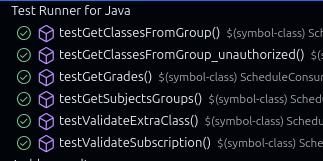
\includegraphics[width=0.55\textwidth]{figures/07_test.png}
    \caption{Pruebas unitarias e integración del servicio schedule-consumer-service}
    \label{test}
\end{figure}

\section{Sprint 4}

En este punto ya tenemos un backend sólido y funcional, con servicios que permiten gestionar usuarios, autenticación, suscripciones a asignaturas y horarios de la UGR. El siguiente paso es desarrollar el frontend de la aplicación, que permitirá a los usuarios interactuar con el sistema de manera intuitiva y visual.
\subsection{Frontend con Angular}
El frontend se desarrolla con Angular (versión 19.0.2), lo que significa que se utiliza TypeScript como lenguaje principal, junto con HTML y CSS para la estructura y el estilo de la aplicación. Angular es un framework de desarrollo web que permite crear aplicaciones de una sola página (SPA) de manera eficiente y escalable.
\subsubsection{Estructura del proyecto}
El proyecto de Angular se organiza en ``components'', ``services'' y ``models'', siguiendo las mejores prácticas de Angular. Los componentes son las unidades básicas de la interfaz de usuario, los servicios se encargan de la lógica de negocio y la comunicación con el backend, y los modelos definen las estructuras de datos utilizadas en la aplicación.
\subsubsection{Comunicación con el backend}
La comunicación con el backend se realiza a través de servicios que utilizan \texttt{HttpClient} de Angular para hacer peticiones HTTP a los diferentes \textit{endpoints} del API Gateway. Estos servicios manejan la autenticación mediante tokens JWT, que se envían en las cabeceras de las peticiones para identificar al usuario y su rol. Tanto el ``access\_token'' como el ``refresh\_token'' se almacenan en el almacenamiento local del navegador, lo que permite mantener la sesión del usuario activa entre recargas de página.

Además, también se ha hecho uso de ``Observables'' para manejar las respuestas del backend de manera asíncrona, lo que permite una experiencia de usuario más fluida y reactiva. Los servicios se encargan de transformar los datos recibidos del backend en objetos que pueden ser utilizados por los componentes de la interfaz de usuario.

Cada vez que se hace una petición al backend se hace uso de un ``Interceptor'' de Angular, este adjunta el token de acceso a la cabecera Authorization de casi todas las solicitudes salientes. Sin embargo, excluye ciertas rutas relacionadas con la autenticación inicial o el refresco de tokens (como /auth/login o /auth/refresh) para evitar bucles o requisitos innecesarios.
Si una solicitud protegida se realiza sin un token de acceso, el interceptor redirige al usuario a la página de login y lanza un error. Su función más importante es el manejo de tokens de acceso expirados: si una API devuelve un error 401, el interceptor intenta refrescar el token usando el token de refresco. Si el refresco es exitoso, actualiza el token de acceso y reintenta la solicitud original. Si el token de refresco también ha expirado, elimina ambos tokens, redirige al usuario al login y reporta un error. Para otros tipos de errores HTTP, simplemente los propaga.
\subsubsection{Rutas y navegación}
El enrutamiento se gestiona mediante el módulo de enrutamiento de Angular, que permite definir rutas para cada componente de la aplicación. Esto facilita la navegación entre diferentes vistas y componentes sin necesidad de recargar la página completa, lo que mejora la experiencia del usuario. Además, se implementa un sistema de guardias de ruta para proteger las rutas que requieren autenticación, asegurando que solo los usuarios con un token JWT válido puedan acceder a ellas.
\subsubsection{Interfaz de usuario}
La interfaz de usuario se ha desarrollado únicamente con HTML, CSS y Tailwind CSS, sin utilizar librerías de componentes adicionales. Esto permite un mayor control sobre el diseño y la apariencia de la aplicación, adaptándola a las necesidades específicas del proyecto. Se han creado componentes reutilizables para las diferentes secciones de la aplicación, como formularios de inicio de sesión, registro, suscripciones y visualización de horarios.
A continuación se muestran en las siguientes figuras (~\ref{login} , ~\ref{calendario} , ~\ref{sincro} , ~\ref{suscripciones} , ~\ref{eventos}) las páginas principales de la aplicación que incluyen el inicio de sesión, la página principal del calendario,la página de sincronización, la página de suscripciones y la página de eventos.

\begin{figure}[H]
    \centering
    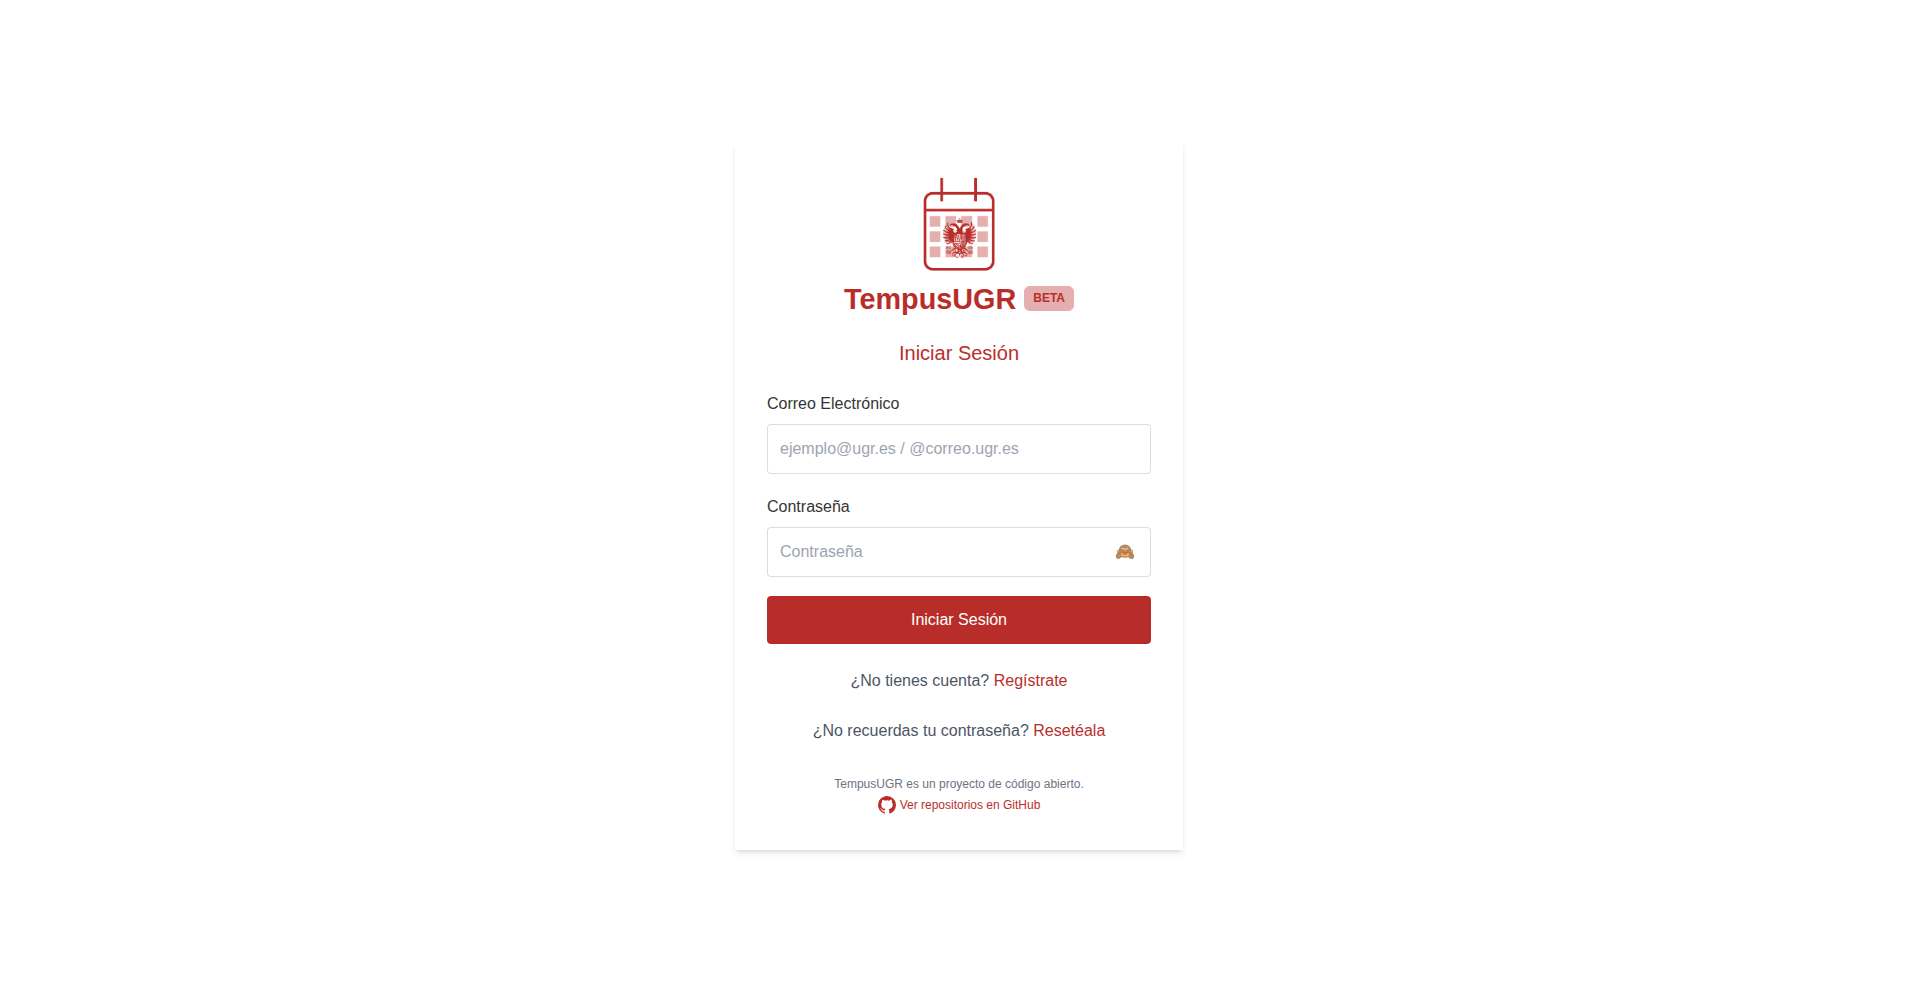
\includegraphics[width=1\textwidth]{figures/07_inicio.png}
    \caption{Página de inicio de sesión}
    \label{login}
\end{figure}
\begin{figure}[H]
    \centering
    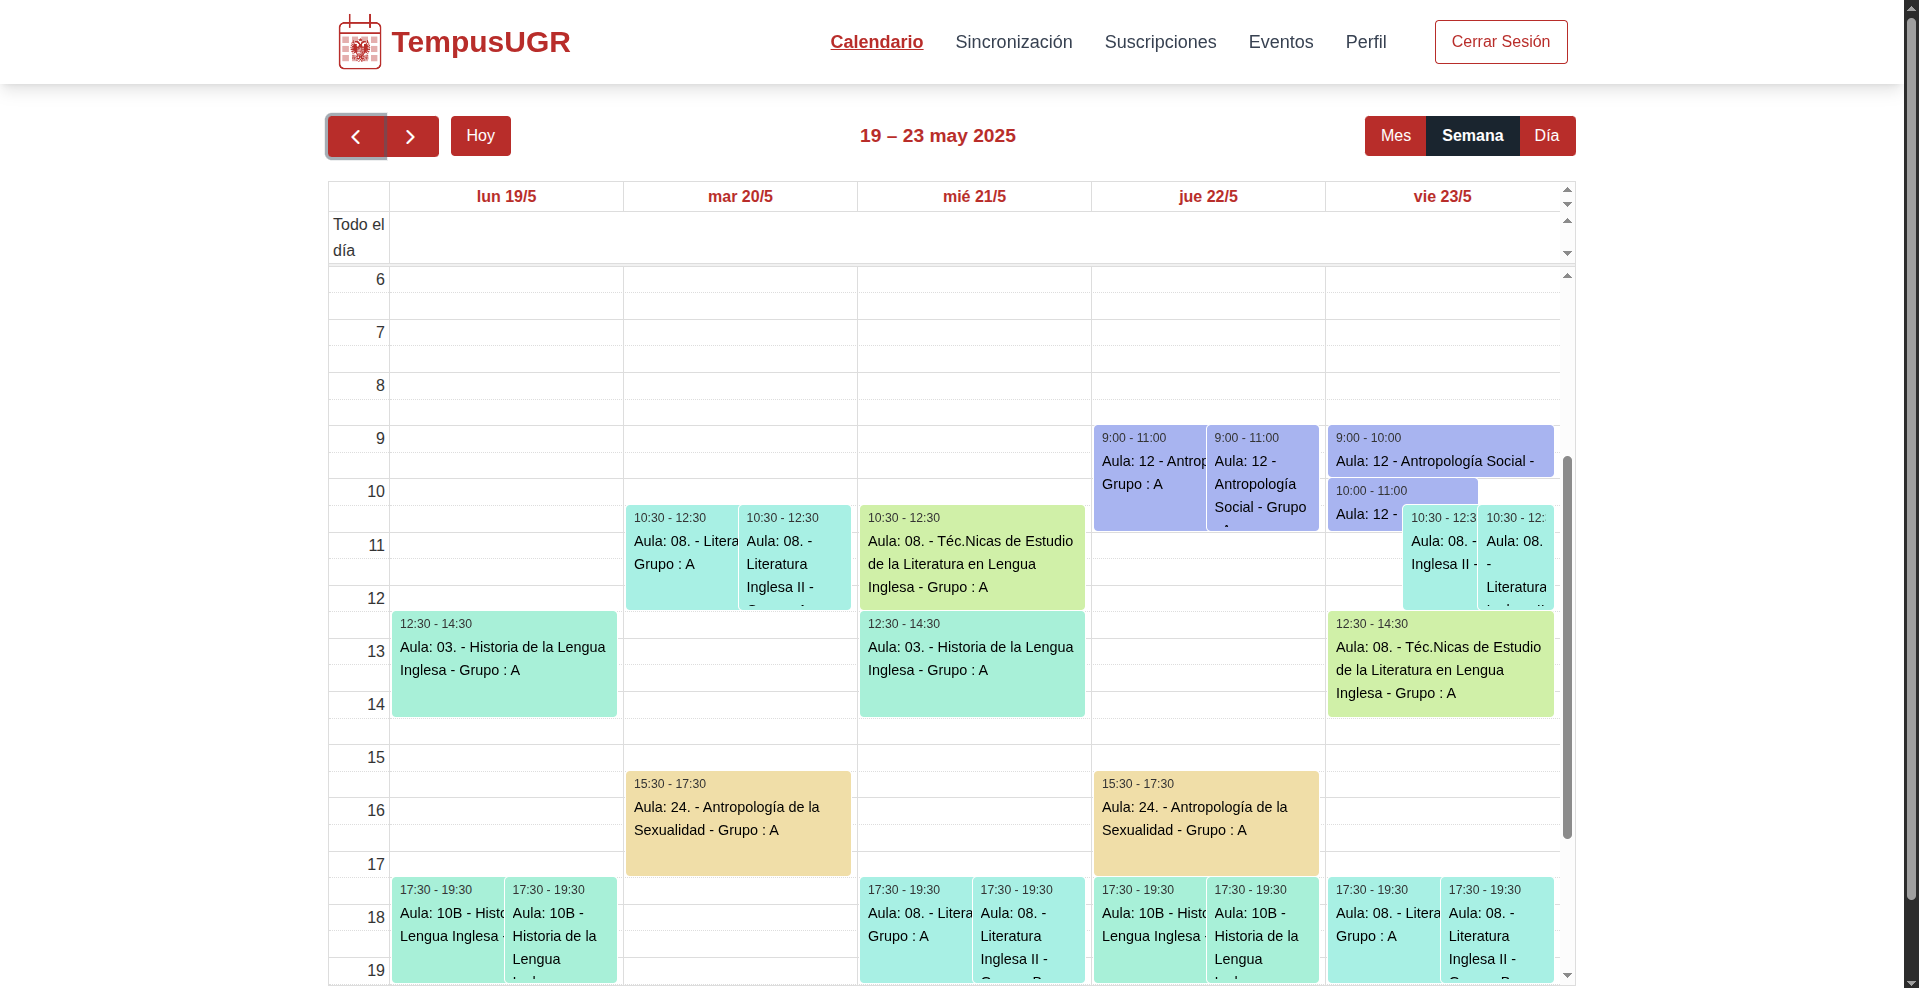
\includegraphics[width=1\textwidth]{figures/07_calendario.png}
    \caption{Página principal del calendario}
    \label{calendario}
\end{figure}
\begin{figure}[H]
    \centering
    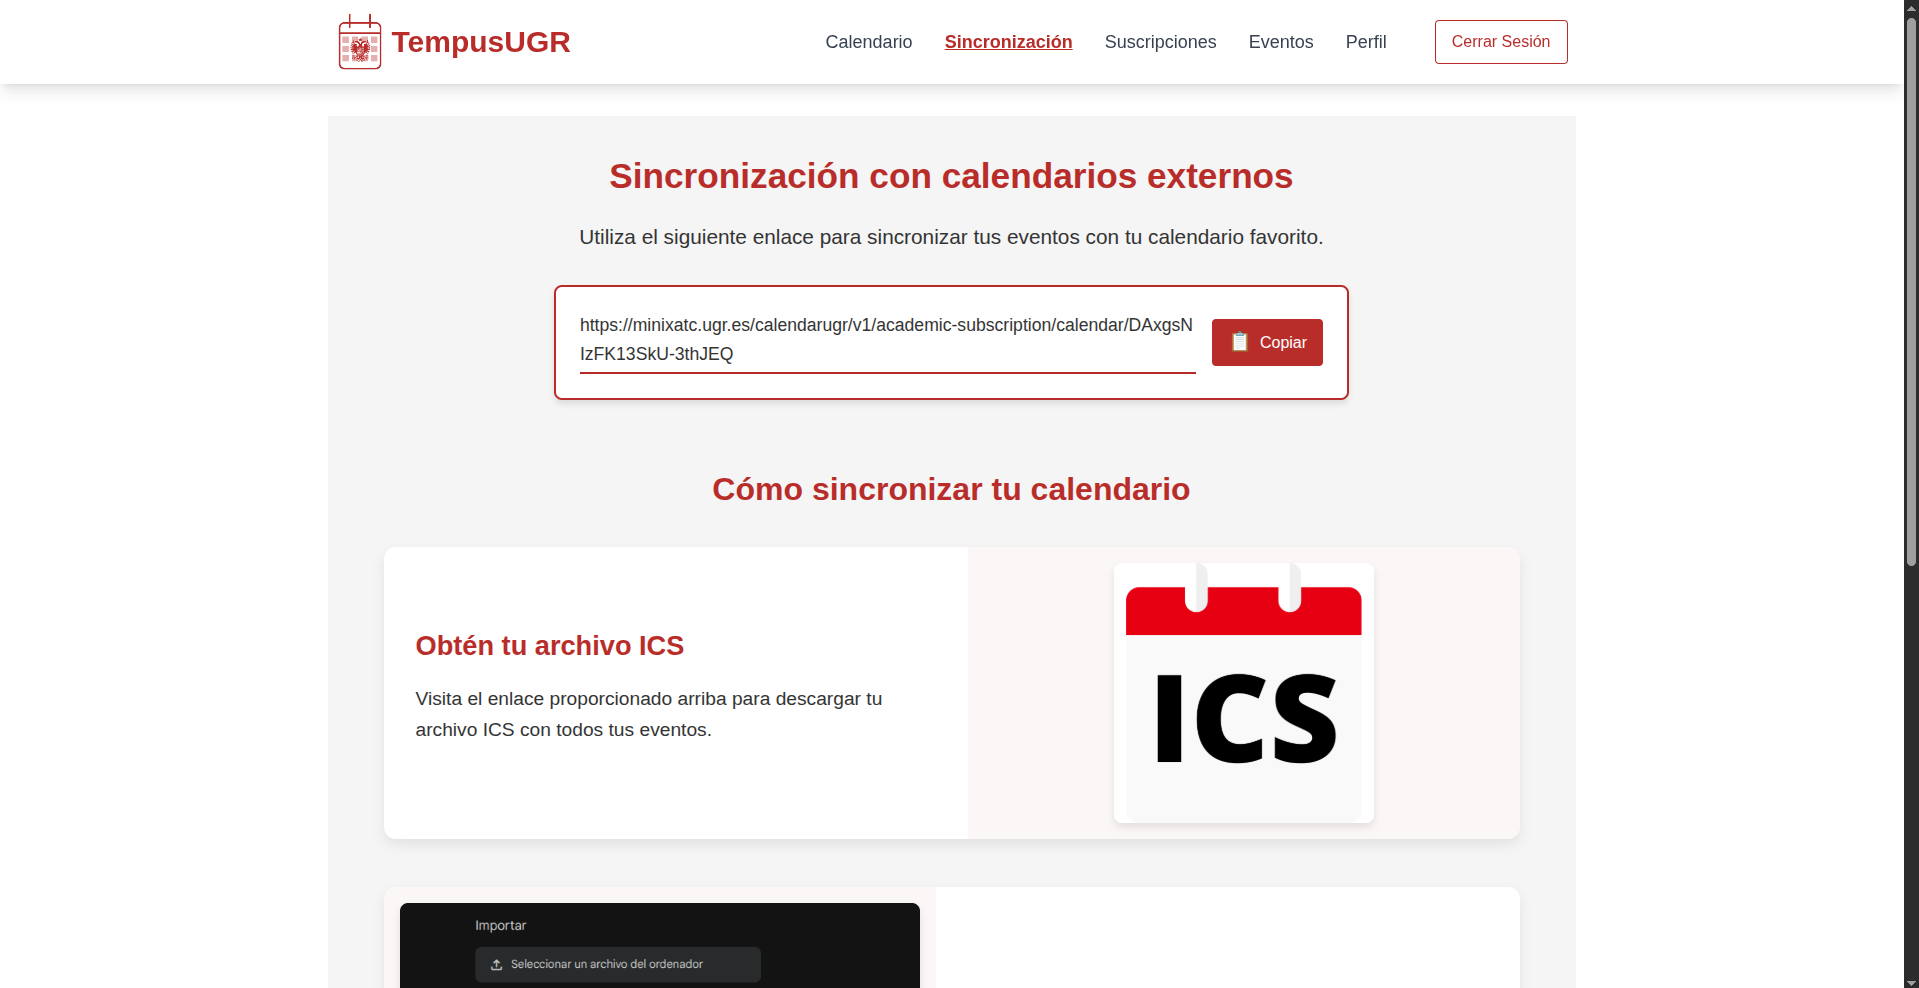
\includegraphics[width=1\textwidth]{figures/07_sincro.png}
    \caption{Página de sincronización con Google Calendar}
    \label{sincro}
\end{figure}
\begin{figure}[H]
    \centering
    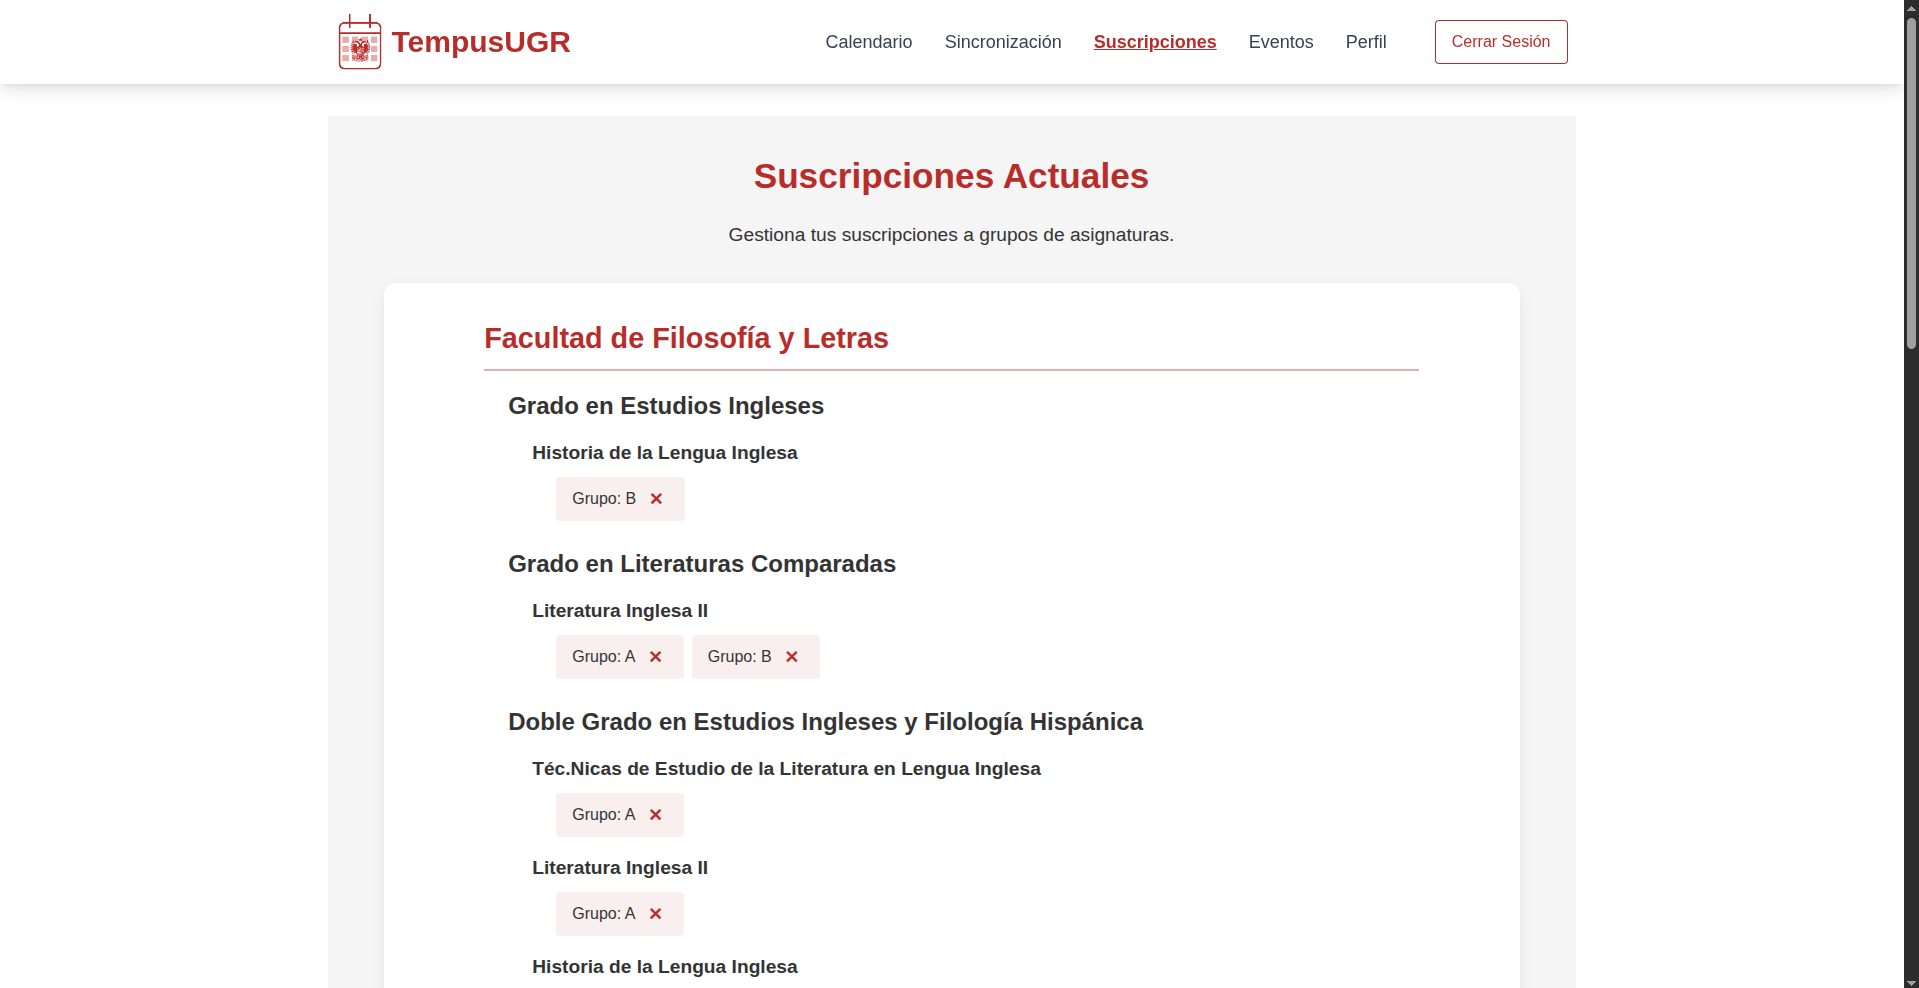
\includegraphics[width=1\textwidth]{figures/07_suscripciones.png}
    \caption{Página de suscripciones a asignaturas}
    \label{suscripciones}
\end{figure}
\begin{figure}[H]
    \centering
    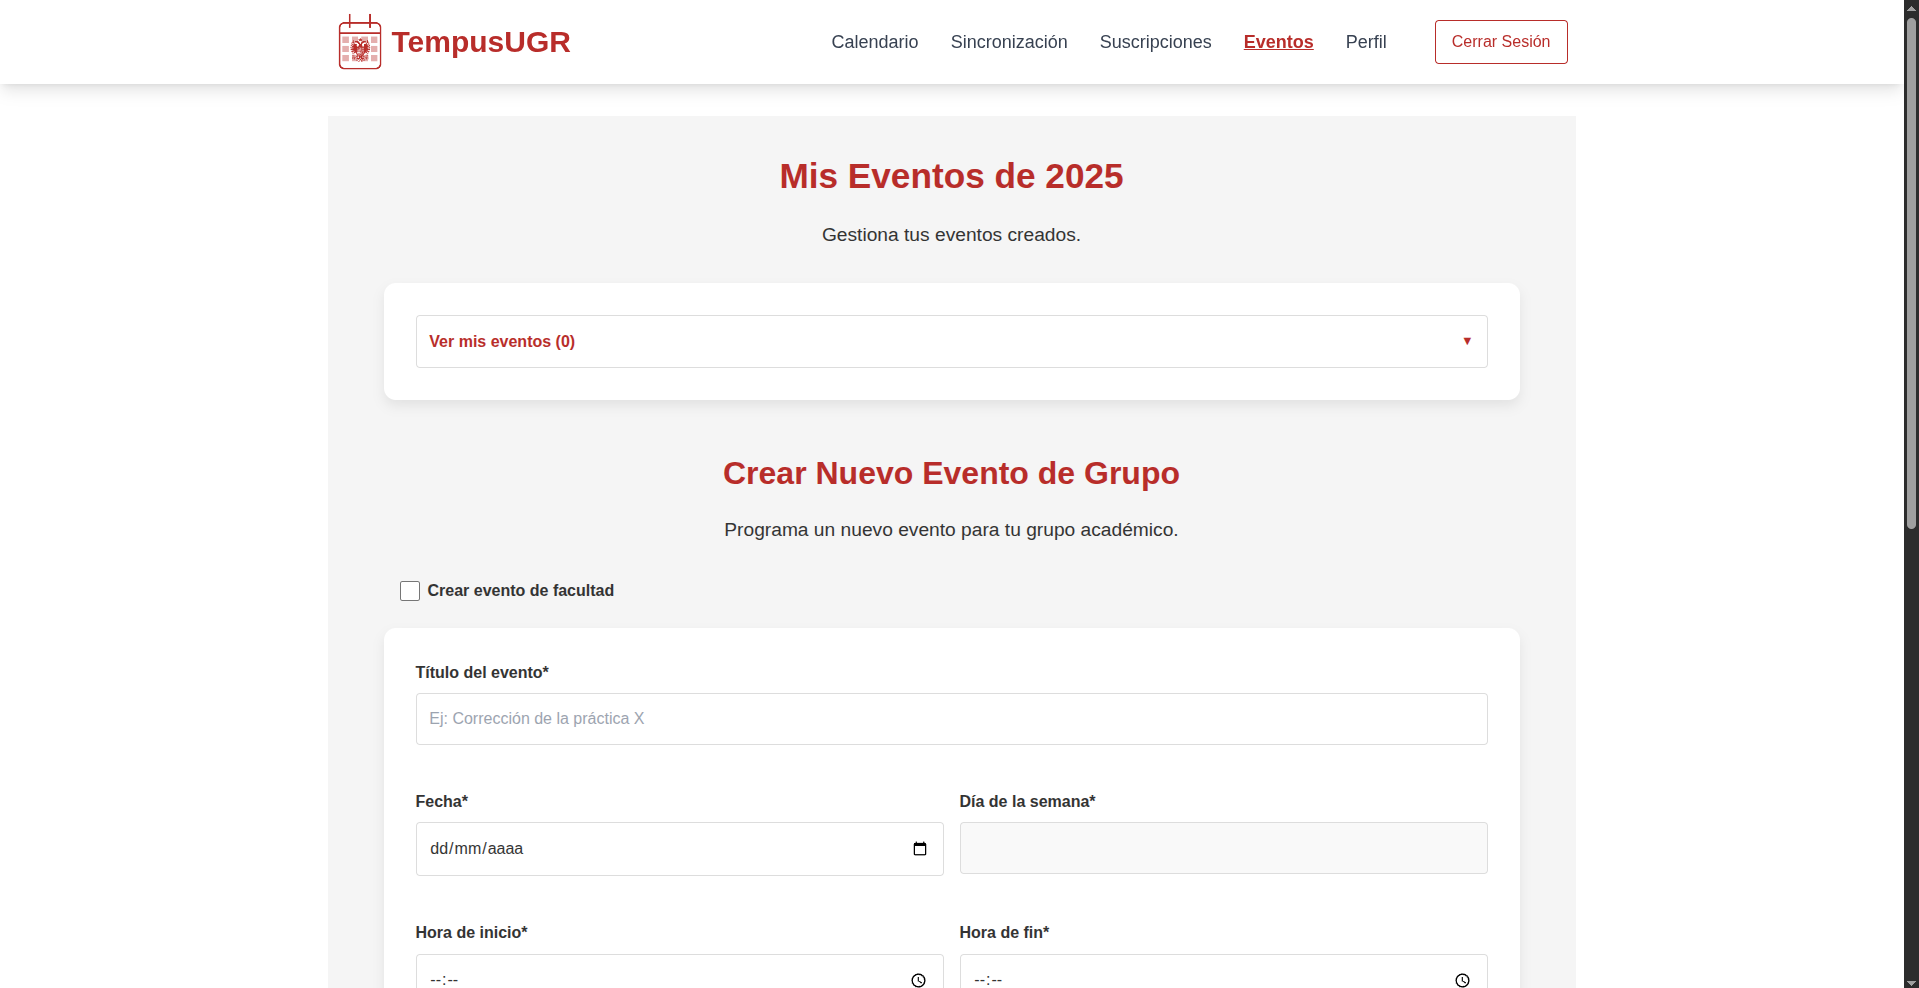
\includegraphics[width=1\textwidth]{figures/07_eventos.png}
    \caption{Página de eventos de grupo y facultad}
    \label{eventos}
\end{figure}

\subsubsection{Suscripción a las asignaturas de un profesor}
Al principio de este sprint se ajustaron tanto el ``Backlog'' como el ``Sprint Backlog'' para incluir la posibilidad de que un profesor pueda suscribirse a las asignaturas que imparte automáticamente buscando su nombre. Esta es una funcionalidad que se detectó como necesaria durante el desarrollo del frontend, ya que tenemos la información necesaria para poder implementarla, y es una funcionalidad que se espera que sea utilizada por los profesores de la UGR.
\newline
Al tener todos los servicios necesarios implementados, y funcionalidades similares ( obtener clases según grado, obtener todos los grados ...), no costó mucho tiempo y cambios significativos en el código. Se implementó un nuevo \textit{endpoint} en el servicio \texttt{schedule-consumer-service} que permite obtener las asignaturas de un profesor a partir de su nombre, y se añadió una nueva funcionalidad en el servicio \texttt{academic-subscription-service} que permite suscribirse a varias asignaturas a la vez.
Por otra parte en el apartado ``suscripciones'' se añadió un ``dropdown'' que sólo podrán visualizar los profesores y administradores, que les permitirá buscar por su nombre y suscribirse a todas sus asignaturas directamente.

\section{Sprint 5}

Las últimas tres semanas del desarrollo se destinaron a depurar y arreglar errores tanto en el frontend como en el backend. Además antes de comenzar este sprint también se hicieron modificaciones en el ``Backlog'' y el ``Sprint Backlog'' para añadir la funcionalidad de ``reseteo de contraseña''. Esta se detectó al hacer pruebas exhaustivas del sistema. Al pretender desplegar el sistema y que esté preparado para su uso, esta es una funcionalidad que se considera esencial para cualquier sistema de gestión de usuarios, y que no se había implementado hasta ahora.
\newline
Al contrario que en el sprint anterior, esta funcionalidad sí requiere de varios pasos para su implementación puesto que requiere, en el caso del backend, un endpoint para solicitar el reseteo, lógica para poder mandar un correo al usuario, y otro endpoint para modificar su contraseña, mientras que en el frontend se requerían un modal para solicitar un correo de contacto, y una página para establecer la nueva contraseña.

En todos los sprint, además de desarrollo, se ha destinado parte del tiempo para ir completando la documentación (diagramas, esquemas, redacción, etc), pero en este sprint se pretende completar la memoria.
\newline
Además al final, y tras este sprint, se despliega el sistema en un servidor de producción, y se realizan pruebas de carga y estrés para comprobar que el sistema es capaz de soportar un número elevado de usuarios concurrentes. Este apartado se desarrolla con más detalle en el apartado de ``Despliegue''\ref{cap:despliegue}.